\documentclass[12pt,notitlepage]{article}
\usepackage{graphicx}
\usepackage{verbatim}
\usepackage[portuguese]{babel}
\usepackage[utf8]{inputenc}
\usepackage[hmargin=2cm,vmargin=3.5cm,bmargin=2cm]{geometry}
\usepackage{multicol}
\usepackage{hyperref}
\usepackage{enumerate}



\begin{document}

%%%CAPA%%%
\begin{titlepage}
\begin{figure}
\centering

\includegraphics[scale=0.5]{logo.pdf}
\end{figure}



\begin{center}

Escola de Engenharia \\~  Departamento de Informática \\~ \\~ Licenciatura em Engenharia Informática \\~ \\~ \\~  \\~ \\~ \\~ \\~ \\~ \\~ \\~


{\Huge Projecto Java - FitnessUM }
\\~ \\~ \\~ \\
Programação Orientada aos Objectos
  \vfill

\begin{figure}[h]
\centering

\end{figure}

\begin{figure}[h]
\centering
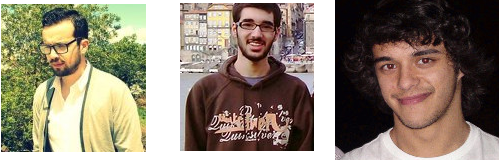
\includegraphics[scale=0.6]{autores.png}
\end{figure}

69303 ~~~~~~~~~~~~~~~~~~ 66822 ~~~~~~~~~~~~~~~~~~~~~ 69854   \\~ Bruno Pereira  ~~~~~~~~ Miguel Guimarães ~~~~~~~João Mano  \\~ \\~ \\~ \\~ \\~ \\~ Braga, Junho de 2014
\end{center}
\end{titlepage}




\tableofcontents
\newpage
\listoffigures
\newpage


\section{Estrutura da aplicação}

\subsection{Actividades}
Foram definidas as seguintes actividades desportivas para a nossa aplicação:
\begin{multicols}{2}
\begin{itemize}
\item Yoga
\item Aerobics
\item Swimming
\item IndoorCycling
\item Handball
\item Basketball
\item TableTennis
\item Boxing
\item Badminton
\item VolleyBallIndoor
\item Football
\item VolleyBallBeach
\item Running
\item Skating
\item Saling
\item Walking
\item Tennis
\item Skiing
\item Cycling
\item MountainBiking
\item Orienteering
\item Snowboarding
\item Polo
\end{itemize}
\end{multicols}

Para a implementação destas actividades foi usada a seguinte estrutura:



\begin{figure}[ht]
\centering
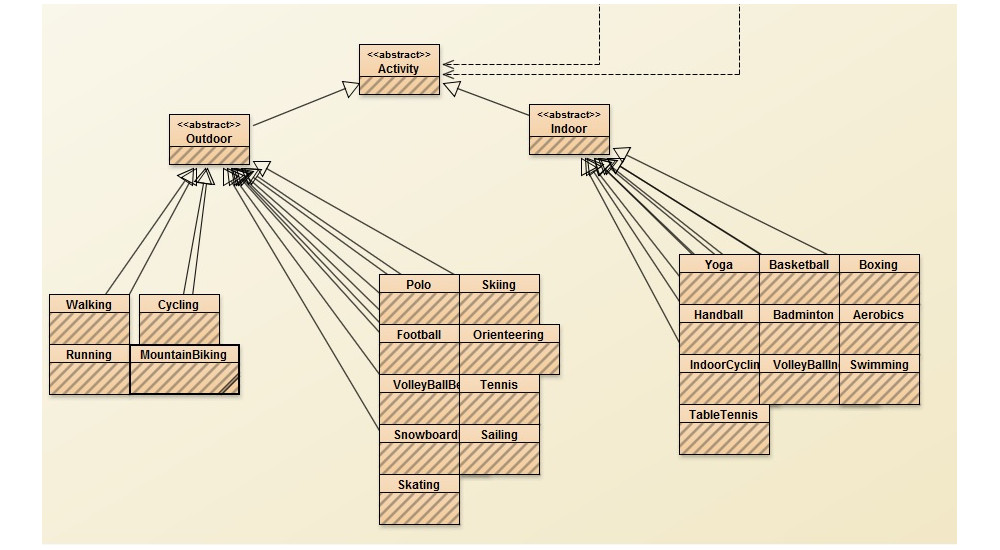
\includegraphics[scale=0.5]{Activity2.jpg}
\caption{Estrutura das actividades}
\label{fig:actividades}
\end{figure}


\subsubsection{Classe abstracta Activity}

Esta é a classe mais abstracta que contem o conceito de actividade. Contém variáveis comuns a todas as actividades:
\begin{itemize}
\item \textit{String name}, nome da actividade criada.
\item \textit{GregorianCalendar date}, data de quando se realizou a actividade.
\item \textit{double timeSpent}, tempo gasto na actividade.
\item \textit{double calories}, campo preenchido pela aplicação de uma fórmula.
\end{itemize}
tal como os construtores, \textit{getters} e \textit{setters}.


\subsubsection{Indoor,Outdoor e actividades desportivas}
Todas as actividades desportivas tem um aspecto importante,o clima caso sejam praticadas ao ar livre.\\
Devido a este aspecto foram criadas duas classes abstractas,subclasses de \textit{Activity},para essa distinção.
\begin{itemize}
\item Outdoor,contém a variável: \textit{String weather}
\item Indoor
\end{itemize}

Todas as actividades desportivas são subclasses de \textit{Indoor} ou \textit{Outdoor} como exemplificado na figura \ref{fig:actividades}.


\subsubsection{Comparadores e Interfaces}
Para organizar as actividades criaram-se dois tipo de comparadores,como exemplificado na figura \ref{fig:CompareActivity}

\begin{itemize}
\item CompareActivity- Compara a actividade pela data da realização da mesma.
\item CompareActivityByTime- Compara a actividade pelo tempo gasto na realização desta.
\end{itemize}

Depois de uma análise às actividades desportivas, ficou claro que para certas actividades deviam-se registar distancias e que para outras registar pontuações,neste seguimento foram criadas as seguintes interfaces:

\begin{itemize}
\item UserVs-Interface de métodos relacionados com pontos(pontos próprios e pontos do adversário)
\item Distance -Interface de métodos relacionados com actividades de distancia.
\item VerticalDistance- Interface de métodos relacionados com actividades de distancia vertical
\end{itemize}

\newpage
\begin{figure}[ht]
\centering
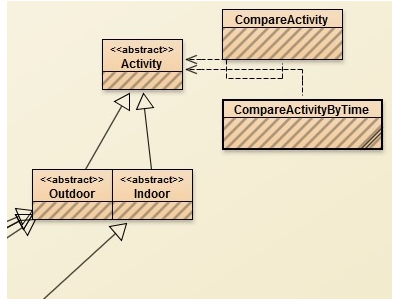
\includegraphics[scale=0.7]{ComparadorActivity.png}
\caption{Comparador CompareActivity}
\label{fig:CompareActivity}
\end{figure}

\begin{figure}[ht]
\centering
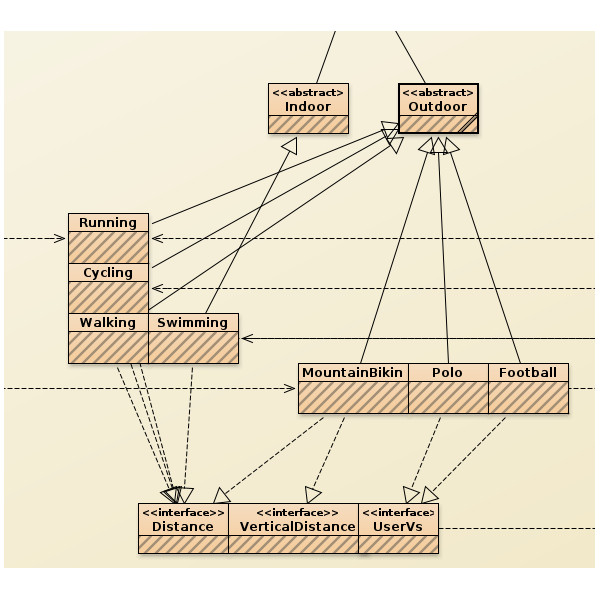
\includegraphics[scale=0.4]{interfaceAct.jpg}
\caption{Exemplo de actividades que implementam as interfaces Distance,VerticalDistance e UserVs}
\end{figure}
~\\~\\





\subsection{Utilizadores}
Para distinguir utilizadores regulares de administradores criou-se a estrutura exemplificada na figura ~\ref{fig:utilizadores}

\begin{figure}[htb]
\centering
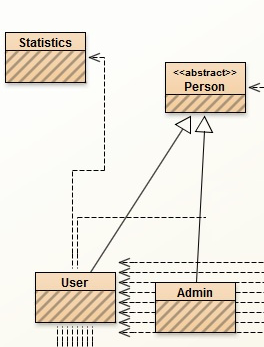
\includegraphics[scale=0.6]{Statsfinalpngg.png}
\caption{Estrutura das classes User e Admin}
\label{fig:utilizadores}
\end{figure}


\subsubsection{Classe abstracta Person}

~\\~
Classe geral para todo tipo de utilizador. As suas variáveis são:
\begin{itemize}
\item \textit{String email};
\item \textit{String password};
\item \textit{String name};
\item \textit{char gender};
\item \textit{GregorianCalendar dateOfBirth};
\end{itemize}

\subsubsection{Classes User e Admin}

As subclasses de Person referem-se a dois possíveis tipos de utilizador, utilizador normal ou utilizador com privilégios de administrador.\\
A classe Admin não tem métodos ou variáveis adicionais, visto que este tipo de utilizador apenas opera sobre a base de dados da aplicação.\\~\\~\\



A classe User adiciona as seguintes variáveis:
\begin{itemize}
\item \textit{int height};
\item \textit{double weight};
\item \textit{String favoriteActivity};
\item \textit{TreeSet$<$Activity$>$ userActivities} - Actividades realizadas pelo utilizador;
\item \textit{TreeSet$<$String$>$ friendsList} - Lista dos amigos do utilizador;
\item \textit{TreeMap$<$String, ListRecords$>$ records} - Lista dos seus recordes pessoais;
\item \textit{TreeSet$<$String messageFriend} - Lista de pedidos de amizade;
\end{itemize}
Respectivos métodos \textit{getters} e \textit{setters}, construtores e métodos auxiliares para a gestão de amigos/pedidos de amizade, recordes pessoais, das suas actividades e estatísticas relevantes. Ainda contém funções auxiliares para a simulação de eventos.

\subsubsection{Comparators}
O tipo Person tem apenas um comparator:
\begin{itemize}
\item ComparePersonByName - que ordena por ordem alfabética do seu nome.
\end{itemize}
\subsubsection{Statistics}

A classe Statistics é usada para mostrar ao utilizador dados relevantes das suas actividades, estes podem ser descriminados por um dado mês ou por um ano. As suas variáveis são:
\begin{itemize}
\item \textit{double timeSpend};
\item \textit{double calories};
\item \textit{double distance};
\end{itemize}
contém os respectivos métodos \textit{getters} e \textit{setters} e construtores.


\subsection{Recordes Pessoais}
Para registar os recordes chegou-se a estrutura da fig ~\ref{fig:recordes}:
~\\
\begin{figure}[h]
\centering
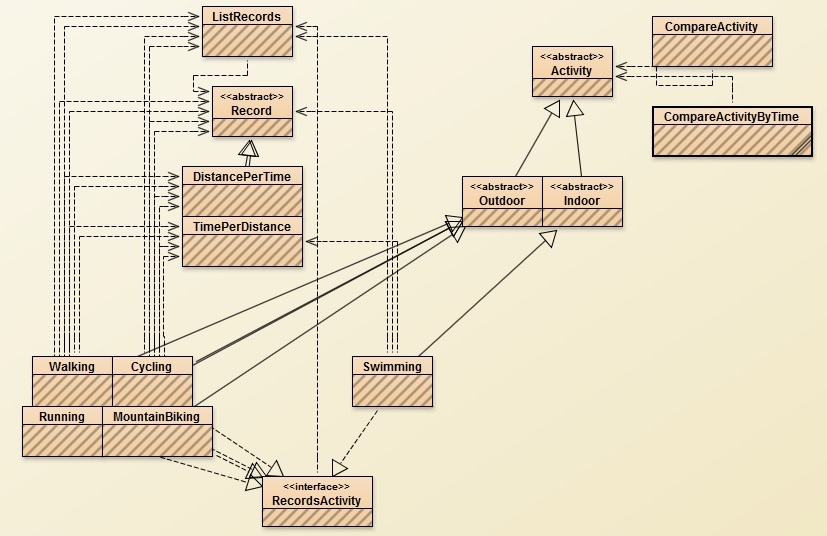
\includegraphics[scale=0.6]{Records.jpg}
\caption{Estrutura dos recordes}
\label{fig:recordes}
\end{figure}


Como se pode verificar na figura ~\ref{fig:recordes}, apenas as seguintes actividades contêm recordes:
\begin{itemize}
\item Running
\item Cycling
\item Walking
\item MountainBiking
\item Swimming
\end{itemize}


\subsubsection{Classe abstracta Record}

Esta classe representa todos os recordes que o utilizador pode bater. Contém apenas uma variável:
\begin{itemize}
\item \textit{String name}-Nome do tipo de recorde a bater(ex: 1km,10 miles,Cooper...)
\end{itemize}
métodos construtores, \textit{getName()} e \textit{isEmpty()} que verifica se esse recorde existe ou não.


\subsubsection{DistancePerTime e TimePerDistance}
Estas classes simbolizam os dois diferentes tipos de recordes.\\

DistancePerTime é um recorde em que o objectivo é fazer a maior distância para um dado tempo.
As suas variáveis são:
\begin{itemize}
\item \textit{double recordTime} - Tempo do recorde;
\item \textit{double distance} - Distância registada;
\end{itemize}
Enquanto que TimePerDistance representa um recorde de menor tempo para uma certa distância.
As suas variaveis sao:
\begin{itemize}
\item \textit{double recordDistance} - Distância do recorde;
\item \textit{double time} - Tempo registado;
\end{itemize}
~\\
Estas duas classes têm os mesmos métodos, no entanto os métodos \textit{update} e \textit{setStatistics}, estão implementados de maneiras diferentes, tendo em conta que em DistancePerTime, quanto maior a distância melhor é o recorde, e no caso do TimePerDistance,  o melhor recorde é o de menor tempo.


\subsubsection{ListRecords}

Classe que agrupa todos os recordes de uma actividade. Tem como variáveis:
\begin{itemize}
\item \textit{String name} - Aqui o nome simboliza o tipo de actividade (Ex: Running, Walking...);
\item \textit{ArrayList$<$Record$>$ recs} - Lista dos recordes;
\end{itemize}
Tem implementado métodos construtores, \textit{getters}, \textit{setters} e ainda um método \textit{updateList()} que aplica a função \textit{update()} a todos os objectos \textit{Record} da lista. (Substitui na lista original caso recorde da segunda lista seja melhor).
\subsubsection{Interfaces}
Nesta fase,visto que nem todas as actividades desportivas implementarem recordes, chegou-se então à conclusão que estas actividades precisam sempre de devolver a lista de recordes registados,então implementou-se a seguinte interface:
\begin{itemize}
\item \textit{RecordsActivity};
\end{itemize}
Que contém o seguinte método:
\begin{itemize}
\item \textit{getListRecords};
\end{itemize}

\subsection{Eventos}
A figura \ref{fig:eventos} representa a nossa estrutura para os eventos.


\begin{figure}[h]
\centering
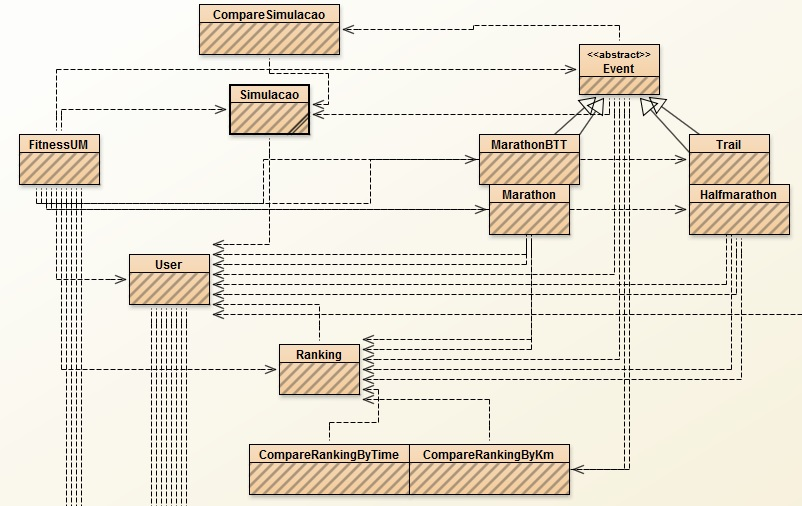
\includegraphics[scale=0.6]{simula.jpg}
\caption{Estrutura dos Eventos}
\label{fig:eventos}
\end{figure}


\subsubsection{Classe abstracta \textit{Event}}
Classe com o conceito mais abstracto de Evento, contém as variáveis:
\begin{itemize}
\item \textit{String name} - Nome do evento;
\item \textit{String tipoActivity} - Tipo de actividade (Running, Walking, ...);
\item \textit{String location} - Onde se realiza a prova;
\item \textit{int maxParticipants} - Número máximo de participantes;
\item \textit{int participants} - Número actual de participantes ;
\item \textit{GregorianCalendar deadline} - Data limite de inscrição;
\item \textit{GregorianCalendar date} - Data de realização;
\item \textit{double duration} - Duração da prova;
\item \textit{TreeSet$<$User$>$ participantsList} - Lista de participantes;
\item \textit{TreeSet$<$Ranking$>$ ranking} - Classificação dos que acabaram a prova;
\item \textit{TreeSet$<$Ranking$>$ desistentes} - Participantes que desistiram da prova;
\item \textit{TreeSet$<$Simulacao$>$ simula} - Informação relevante para simular cada concorrente;
\end{itemize}
respectivos \textit{getters} e \textit{setters} e os vários construtores. Ainda tem métodos auxiliares para, adicionar um \textit{User}, \textit{Ranking} (desistente ou não) e \textit{Simulacao} aos respectivos \textit{Sets} e para mostrar a classificação geral do evento.


\subsubsection{Tipo de Evento}

Subclasses de Evento (\textit{Marathon}, \textit{HalfMarathon}, \textit{MarathonBTT} e \textit{Trail}), todas estas contem mais uma variável \textit{distance}, que nos casos de \textit{Marathon} e \textit{HalfMarathon} são variáveis \textit{final}, porque este tipo de eventos tem distâncias especificas. Não tem métodos auxiliares para além de \textit{getDistance()}.


\subsubsection{Simulação}

Para guardar dados relevantes à simulação de cada utilizador para um evento, foi criada a classe \textit{Simulacao}. A simulação de cada evento é feita actualizando os dados desta classe a cada km.

\begin{itemize}
\item \textit{double tempoGeral} - Tempo acumulado do utilizado na realização da prova.
\item \textit{double tempoMedio} - Tempo médio por km.
\item \textit{int kmDesiste} - Número de km que o utilizador aguenta durante a prova.
\item \textit{User u} - Utilizador associado á simulação.
\end{itemize}
esta classe, para além dos métodos construtores e \textit{getters} e \textit{setters}, contém apenas um método \textit{actualiza}, que simula a passagem de uma distância (passada como argumento), usando o tempo médio por km e aplicando um factor aleatório (usando \textit{Math.random()}.



\subsubsection{Ranking}

Cada evento, para organizar a sua classificação, utiliza duas colecções de objectos da classe \textit{Ranking}. Uma delas, usada para organizar todos os participantes, que concluíram a prova, por ordem de chegada, a outra onde estão os aqueles que não terminaram, organizados por número de quilómetros realizados.

Esta classe usa as seguintes variáveis:
\begin{itemize}
\item \textit{double time} - Tempo de realizado no evento;
\item \textit{int km} - Número de quilómetros realizados;
\item \textit{User athlete} - Utilizador;
\end{itemize}
Das variáveis \textit{time} e \textit{km}, apenas uma irá ter algum valor para cada utilizador, visto que esta classe é usada para ordenar classificações finais, cada pessoa tem ou um tempo de conclusão do evento ou o número do quilómetro em que desistiu. \textit{Ranking} contém os métodos \textit{getters} e \textit{setters} relevantes, construtores, e para além dos métodos essenciais, foram implementados dois métodos \textit{toString} alternativos, para os dois casos.

\subsection{Fórmulas}
Em certos momentos do trabalho surgiu a necessidade de codificar fórmulas.\\
Tal aconteceu para calcular as calorias gastas em cada actividade e para a simulação dos eventos.

\subsubsection{Fórmula das Calorias}
~\\~
\textbf{MET(Metabolic Equivalent of Task)}- É  uma medida fisiológica que expressa o custo energético de cada actividade física.\\
  Sabendo o que MET's representa, e retirando essa medida, para cada actividade ,pelo seguinte quadro: \url{http://www.cdof.com.br/MET_compendium.pdf}\\


Criou-se a seguinte fórmula das calorias para cada actividade:\\

\begin{tabular}{|r|}
  \hline
  \\
 \textbf{Calorias}$=mets * pesoDoUtilizador * (tempoGasto(min) / 60)$\\
 \\
 \hline \hline
\end{tabular}


\subsubsection{Fórmula para a Simulação}

Para inferir um valor médio de minutos/km foi seguido o seguinte raciocínio:\\
\begin{enumerate}
\item Calculou-se um tempo médio em função do evento.
\item Contou o número de actividades praticadas do tipo do evento(ex: evento-Marathon,tipo do evento-Running).
\item Aplicou-se a fórmula idealizada.
\end{enumerate}
~\\~
Para calcular o tempo médio em função do evento,fez-se uma distinção entre MarathonBTT e os outros eventos.\\~\\
Para o evento \textbf{MarathonBTT} percorreu-se todas as actividades do tipo "MountainBiking" e para cada uma delas:
\begin{itemize}
\item Calculou-se um factor, de 0 a 1, em função do parâmetro VerticalDistance(quanto maior,maior é o factor).
\item Somou-se a distancia com o acumulado da mesma.
\item Somou-se o acumulado do tempo com o tempo gasto$/$ distancia feita.
\end{itemize}

No fim calcula-se o tempo médio total em função do tempo médio calculado com o factor médio e distancia média realizadas nas actividades. \\~

Para os restantes eventos, a ideia foi a mesma,apenas não se usou o factor.\\~

Tendo o tempo médio calculado(tm) a fórmula para o calculo do tempo médio final é a seguinte:\\~\\~
\begin{tabular}{|r|}
  \hline
  \\
 \textbf{tempo }$= tm + (1 *tabWeather(weather)) + (1 * tabTemp(temperatura)) - (nº/ 100) + (age / 100)$\\
 \\
 \hline \hline
\end{tabular}
~\\~\\

tabWeather$->$ método que devolve um factor(de 0 a 1) em função dos seguintes climas:
\begin{itemize}
\item Sol
\item Sol intenso
\item Sol intenso com ventos fortes
\item Chuva
\item Chuva com ventos fortes
\item Chuva intensa
\item Chuva intensa com ventos fortes
\item Trovoada
\item Trovoada com ventos fortes
\item Nublado
\end{itemize}

tabTemp$->$método que devolve um factor (de 0 a 1) em função da temperatura, em graus Celsius.

nº $->$ número de actividades praticadas do tipo do evento.
~\\~\\


Em \textbf{cada km} da simulação o usa-se este tempo calculado e multiplica-se por $(Math.random() + 0.5)$, factor aleatório que aumenta ou diminui o tempo no km do participante.
~\\~\\

Para a possibilidade de um participante do evento  \textbf{desistir num certo Km} foi usada a seguinte estratégia:
\begin{enumerate}
\item Calculou-se a idade do participante.
\item Calculou-se uma probabilidade.
\item Calculou-se o possível km em que desiste.
\end{enumerate}~\\
A probabilidade foi calculada em função da idade:
\begin{itemize}
\item age $<$ 15- factor = Math.random()* 1.5 + 0.1;
\item age $<$ 20- factor = Math.random()* 1.5 + 0.5;
\item age $<$ 25- factor = Math.random()* 1.5 + 0.7;
\item age $<$ 30- factor = Math.random()* 1.5 + 0.85;
\item age $<$ 35- factor = Math.random()* 1.5 + 0.9;
\item age $<$ 40- factor = Math.random()* 1.5 + 0.6;
\item age $<$ 45- factor = Math.random()* 1.5 + 0.5;
\item age $<$ 50- factor = Math.random()* 1.5 + 0.4;
\item age $<$ 55- factor = Math.random()* 1.5 + 0.3;
\item age $<$ 60- factor = Math.random()* 1.5 + 0.2;
\item age $<$ 65- factor = Math.random()* 1.5 + 0.1;
\item age $>=$ 65- factor = Math.random()* 1.5 + 0.05;
\end{itemize}~\\~

Finalmente multiplica-se este factor pela totalidade de km do evento, e se este km for menor que a distancia total do evento,então será o km de desistência do participante.

\section{Considerações finais}

\subsection{Construtores}
Determinadas classes desta aplicação contém construtores que não estão a ser utilizados por nós, foram sendo adicionados enquanto criávamos estas classes, no entanto, mesmo não sendo utilizados, podem ter utilidade futura fora desta aplicação.

\subsection{Variáveis inutilizadas}
Na classe \textit{Event} a variável \textit{duration} nunca é usada, pois, na criação desta classe pensávamos que íamos precisar da duração do evento, como não demos conta da sua inutilidade até estarmos num estado mais avançado do projecto, decidimos simplesmente ignorar esta variável em vez de a remover. O utilizador nunca terá conhecimento da existência deste problema, pois nunca é pedido esta informação e apenas usamos um construtor que a põe a zero.

\subsection{Actualização de estados}
Durante os testes à funcionalidade da FitnessUM, deparamos com o problema de que, ao ser removida uma actividade, a sua informação continuava a ter relevância para as estatísticas e também para os recordes.
Para melhorar a nossa aplicação foi mudada a implementação das estatísticas para apenas mostrar as actividades que ainda estão na aplicação, em vez de serem actualizadas na adição de uma nova actividade.\\
Para os recordes, no entanto, não foi possível implementar uma funcionalidade equivalente por motivos de tempo, e assim os recordes mostrados ao utilizador são os de todas as suas actividades realizadas, mesmo as que foram removidas.

\newpage

\section{Anexos}
\subsection{Imagens da aplicação}

\begin{figure}[h]
\centering
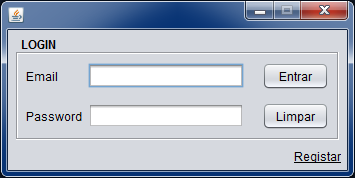
\includegraphics[scale=0.7]{login.png}
\caption{Menu login}
\end{figure}

\begin{figure}[h]
\centering
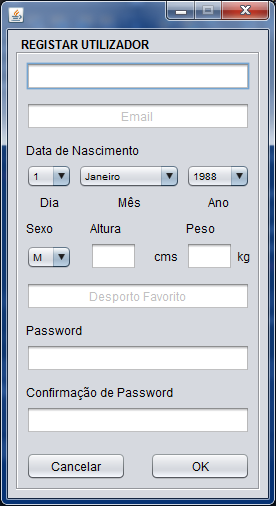
\includegraphics[scale=0.8]{registar.png}
\caption{Menu registar na aplicação}
\end{figure}



\begin{figure}[h]
\centering
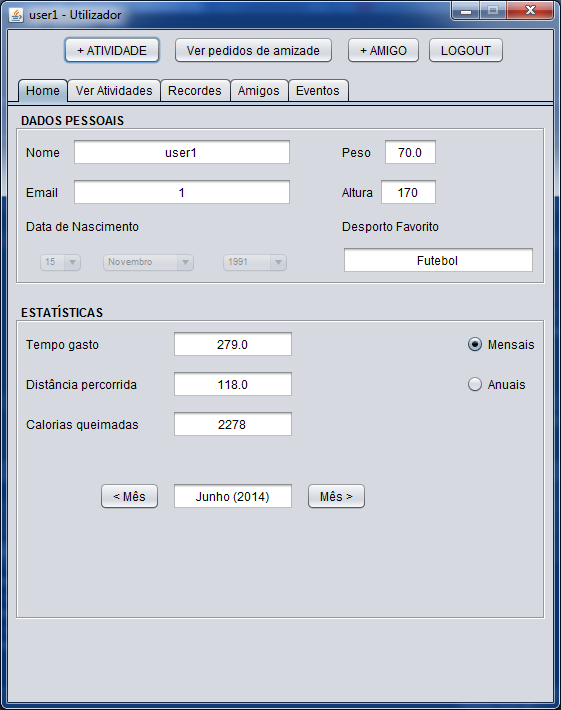
\includegraphics[scale=1]{home.png}
\caption{Menu principal do utilizador}
\end{figure}




\begin{figure}[h]
\centering
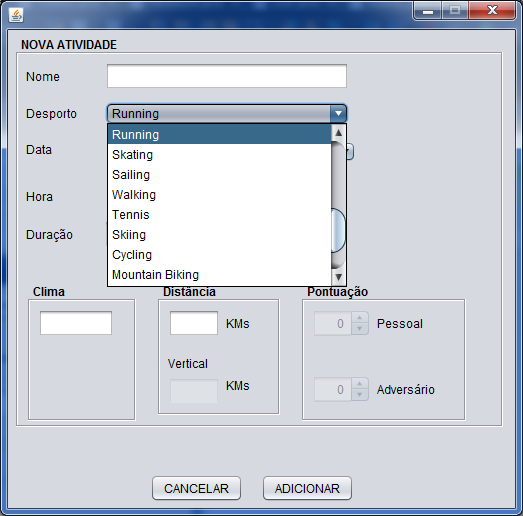
\includegraphics[scale=1]{addActividade.png}
\caption{Menu adicionar actividade}
\end{figure}


\begin{figure}[h]
\centering
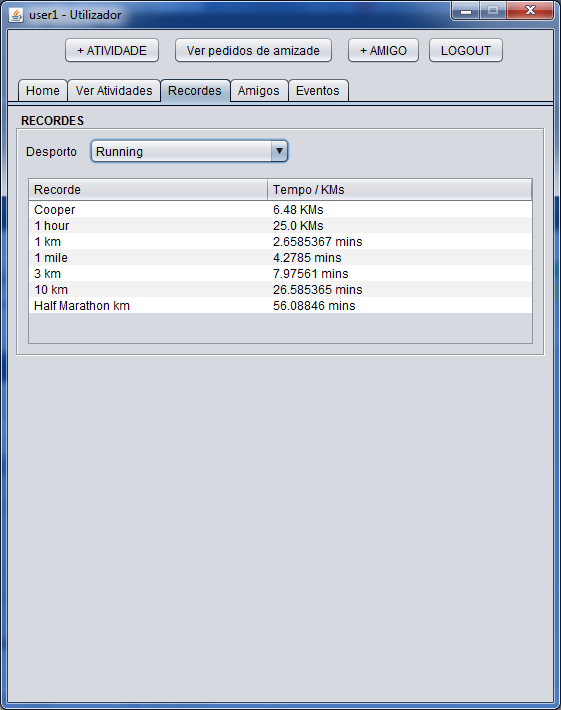
\includegraphics[scale=1]{verRecord.png}
\caption{Menu ver recordes}
\end{figure}



\begin{figure}[h]
\centering
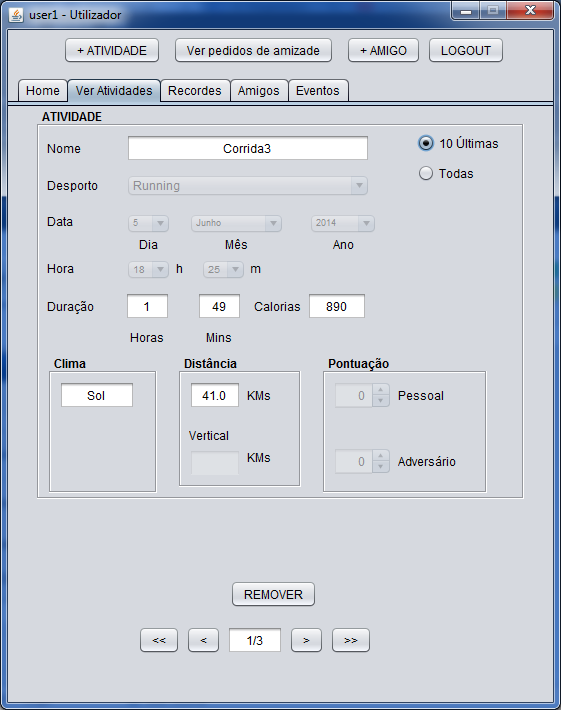
\includegraphics[scale=1]{verActividades.png}
\caption{Menu ver actividades(estatísticas)}
\end{figure}



\begin{figure}[h]
\centering
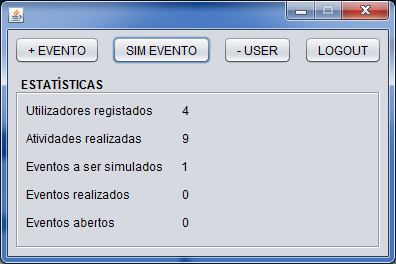
\includegraphics[scale=1]{admin.png}
\caption{Menu administrador}
\end{figure}

\begin{figure}[h]
\centering
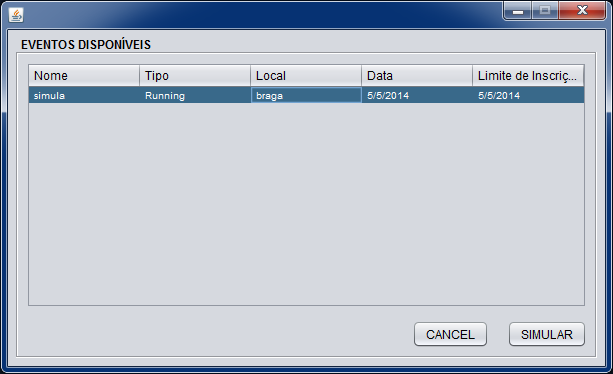
\includegraphics[scale=1]{simularEventosAdmin.png}
\caption{Menu dos eventos para simular}
\end{figure}

\begin{figure}[h]
\centering
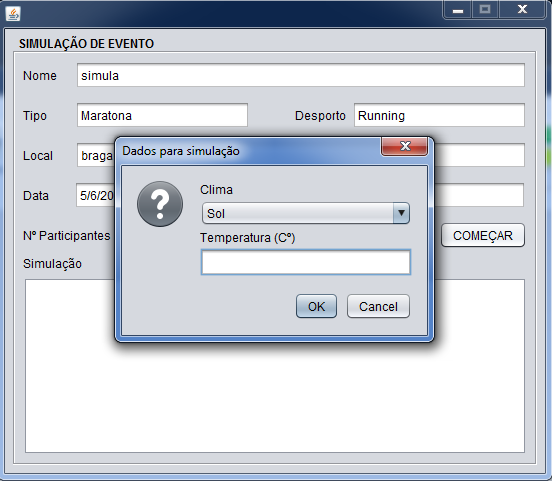
\includegraphics[scale=1]{simTemp.png}
\caption{Menu simulação}
\end{figure}

\begin{figure}[h]
\centering
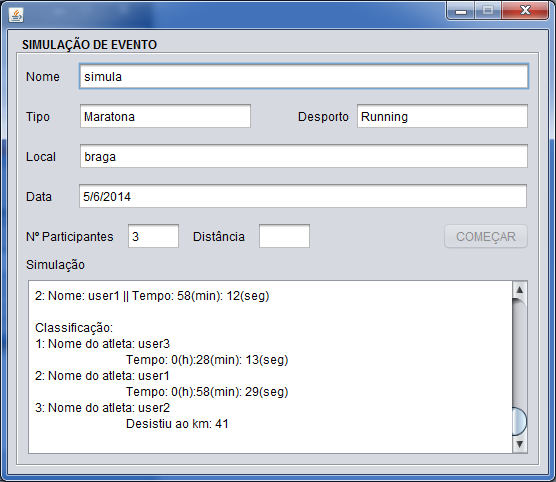
\includegraphics[scale=1]{simulaFinal.png}
\caption{Menu simulação final}
\end{figure}

\end{document}

















